% 本章以根目录 1(1).tex 的背景与研究主线为主体，融合原第一章的技术路线、实现范围及作品优势。
\section{项目背景}

密码技术是网络空间安全的基石，也是电力系统安全稳定运行的重要支撑。随着量子计算技术的发展，Shor 算法对 RSA、椭圆曲线密码等经典公钥机制构成数学结构层面的威胁，Grover 算法则改变密钥搜索等问题的理想查询复杂度；与此同时，电力系统的密码资产与发电、输电、变电、配电、用电各环节业务深度融合，覆盖范围广、终端类型多，增加了资产盘点与量子风险分析的难度。本节从量子计算的威胁机理与电力领域的现实需求两个方面，说明研制电力领域密码资产识别与迁移辅助工具的必要性与紧迫性。

\subsection{量子计算的突破对现有密码体系的影响}

现代密码体系的安全性通常不依赖算法保密，而是建立在特定计算问题的困难性及明确的攻击模型之上：RSA 的安全性与大整数分解相关，Diffie--Hellman 与椭圆曲线密码（ECC）依赖相应群上的离散对数问题，对称密码与杂凑函数则需要分别考察密钥搜索、原像、碰撞及具体构造。经典计算模型下的安全强度不能直接套用于量子计算模型；但量子算法的存在也不等于现实设备已经具备破解工程密码的能力。

量子计算以量子比特为基本信息单元，利用量子态的叠加、纠缠和干涉，通过量子门演化与测量完成计算，能够加速某些经典计算难以求解的问题。1997 年 Shor 正式发表的量子算法与 1996 年 Grover 提出的量子搜索算法，分别从\textbf{数学结构}与\textbf{搜索复杂度}两个层面影响现有密码体系\cite{shor1997,grover1996}。一旦具备足够规模与容错能力的密码学相关量子计算机（Cryptographically Relevant Quantum Computer，CRQC）成为现实，部分传统公钥算法的安全基础将受到根本挑战。Gidney 与 Eker{\aa} 在特定器件错误率、纠错和电路假设下估计，分解 2048 位 RSA 模数约需 2000 万个含噪物理量子比特并运行 8 小时\cite{gidney2021}。这一结果属于资源模型估计，不能据此推定 CRQC 的出现日期。更值得关注的是工程时间尺度：密码改造涉及协议、证书、软件与设备协同，电力行业的长生命周期设备又放大了这一周期，因此资产盘点与迁移准备应提前开展。

Shor 算法通过周期寻找等量子计算步骤，在多项式时间内求解整数分解与离散对数问题，威胁 RSA、ECDSA、ECDH、SM2 等传统公钥机制的数学基础\cite{shor1997,ec-shor}。若相关攻击能力达到实际参数规模，受影响的密钥协商与公钥加密可能使已保存的历史密文暴露；签名机制失效则可能导致设备身份与控制指令签名被伪造，影响证书体系的信任基础。这属于\textbf{算法数学基础层面的风险}，单纯增大传统密钥参数并不改变相关问题可被 Shor 算法在多项式时间求解的性质。长期防护需要结合适用标准，评估后量子密码（Post-Quantum Cryptography，PQC）及经过设计和验证的混合迁移路线。

Grover 算法给出无序搜索的平方加速，将理想查询复杂度由 $O(N)$ 降至 $O(\sqrt{N})$。对于 $k$ 位对称密钥穷举，常用的理论量级比较为 $2^k$ 与 $2^{k/2}$；实际攻击成本还取决于可逆电路、纠错、深度和并行条件\cite{pqc-faq}。杂凑原像与碰撞属于不同问题，不能把 MD5、SHA-1、SHA-256、SM3 的全部安全性质一概称为“强度减半”。DES、RC4 的经典弱点以及 MD5、SHA-1 的碰撞缺陷，也不能仅靠增加参数消除。因此，\textbf{传统公钥机制应优先开展迁移评估，对称与杂凑机制则应结合参数、用途和经典缺陷分别处理}。各类影响归纳如表~\ref{tab:quantum-threat-map}；SM9 等在此用于背景讨论，不等于本文扫描器的已验证识别标签。

\begin{table}[htbp]
  \centering\small
  \caption{量子算法对主要密码体制的影响与评估要点}
  \label{tab:quantum-threat-map}
  \begin{tabularx}{\linewidth}{@{}p{2.6cm}p{2.9cm}p{1.3cm}X@{}}\toprule
    密码体制 & 主要计算问题 & 量子算法 & 评估要点\\\midrule
    RSA & 大整数分解 & Shor & 传统公钥风险；增大模数不改变问题的量子可解性质。\\
    DSA / ECDSA & 有限域或椭圆曲线离散对数 & Shor & 签名私钥可能被求解，需评估身份与信任链迁移。\\
    DH / ECDH & 相应群上的离散对数 & Shor & 密钥协商受威胁，应关注长期机密数据的先存后解风险。\\
    SM2 / SM9 & 椭圆曲线及配对相关群上的离散对数 & Shor & 应开展传统公钥机制的迁移评估。\\
    AES-128 / SM4 & 128 位密钥搜索 & Grover & 理想查询量级约为 $2^{64}$；仍需考虑实际攻击成本与用途。\\
    AES-256 & 256 位密钥搜索 & Grover & 理想查询量级约为 $2^{128}$；还需检查模式与密钥管理。\\
    DES / 3DES / RC4；MD5 / SHA-1 & 密钥搜索、统计攻击或碰撞 & 分类讨论 & 已有经典缺陷或退役要求，按具体用途安排替换。\\
    SHA-256 / SM3 & 原像与碰撞搜索 & 分类讨论 & 原像理想查询量级约为 $2^{128}$；碰撞与认证构造另行分析。\\\bottomrule
  \end{tabularx}
\end{table}

SM4 标准规定的密钥长度固定为 128 位，不存在可在本文直接采用的“SM4-256”标准实例\cite{gbt32907}。表中的理论量级用于说明风险来源，不能从算法名称直接推导完整系统的安全结论。

% 配图说明：使用编号 PNG 的原创时间示意，标明推演条件与来源，不将示意当作实测。
\begin{figure}[htbp]
    \centering
    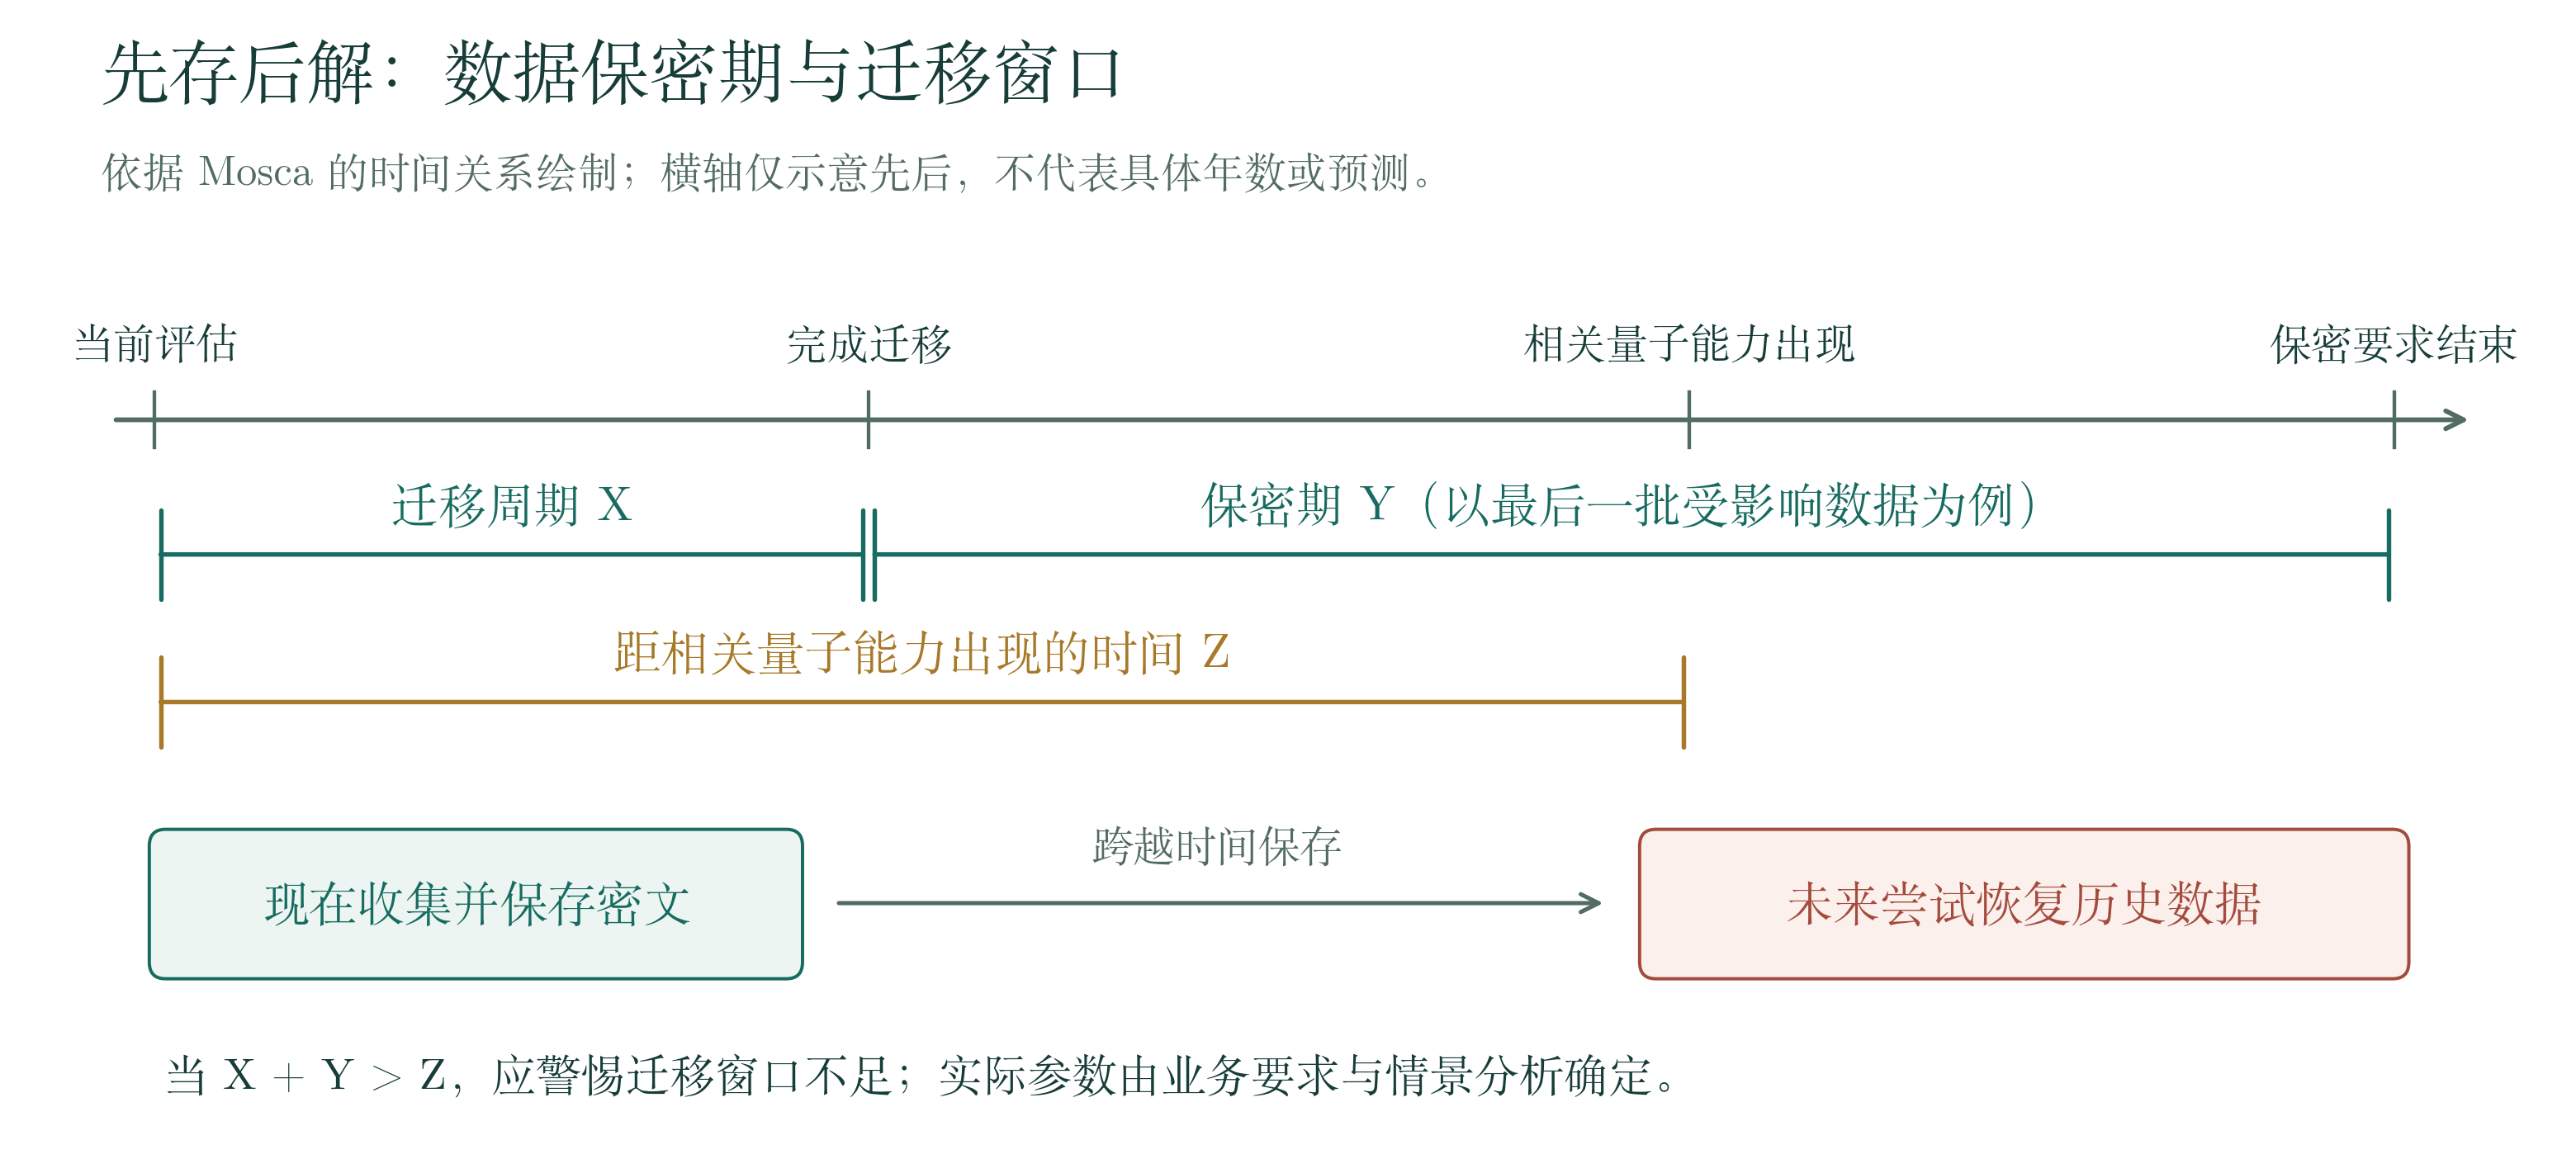
\includegraphics[width=\linewidth]{18-harvest-now-decrypt-later.png}
    \caption{先存后解的时间关系。依据 Mosca 的迁移窗口讨论绘制\cite{mosca2018}；未来量子能力的出现时点仅为示意。}
    \label{fig:gri-timeline}
\end{figure}

在工程评估中，具有指导意义的威胁模型是\textbf{先存后解}（Harvest Now, Decrypt Later，HNDL）：如图~\ref{fig:gri-timeline} 所示，攻击者现在收集并保存受影响机制保护的密文，待未来具备相关量子能力时尝试恢复历史数据。这使未来解密能力成为当前数据保护需要考虑的风险，但不表示本文已观察到实际解密损失。Mosca 提出的时间关系可用于判断迁移窗口：设 $X$ 为完成迁移所需的时间，$Y$ 为数据需要继续保持机密的年限，$Z$ 为从评估时点到相关量子能力出现的时间，若

\begin{equation}
    X + Y > Z,
    \label{eq:mosca}
\end{equation}

则需要警惕在迁移与保密要求尚未同时满足时，受影响数据已经暴露于未来解密能力的风险\cite{mosca2018}。电力系统不同业务的保密期、可升级性与检修窗口并不相同，应分别确定 $X$ 与 $Y$，并对不确定的 $Z$ 做情景分析，而不能统一指定“所有电力数据保密十至二十年”或固定的量子威胁到来日期。

为应对上述威胁，NIST 于 2024 年 8 月发布首批后量子密码标准，包括 FIPS 203（ML-KEM）、FIPS 204（ML-DSA）与 FIPS 205（SLH-DSA）\cite{nistfips203,nistfips204,nistfips205}。迁移时间安排方面，本文引用的 NIST IR 8547 为 2024 年发布的\textbf{初始公开草案}，提出对相关量子脆弱公钥算法在 2030 年前后进入弃用阶段、到 2035 年不再允许用于相应保护用途的规划\cite{nistir8547}。具体时间与范围应按算法、参数、用途及后续正式文件核对，不能表述为已经对全球电力系统生效的强制期限。IEC 62351 系列为电力系统数据与通信安全提供行业标准背景\cite{iec62351}。图~\ref{fig:pqc-timeline} 将已发布标准、草案规划节点与项目迁移活动并列展示。对我国电力行业而言，算法选用与迁移还需满足适用的商用密码制度、产品要求和业务协议约束，准确识别现有密码资产及其用途是分层迁移的前提。

% 配图说明：使用编号 PNG 的原创时间示意，标明推演条件与来源，不将示意当作实测。
\begin{figure}[htbp]
    \centering
    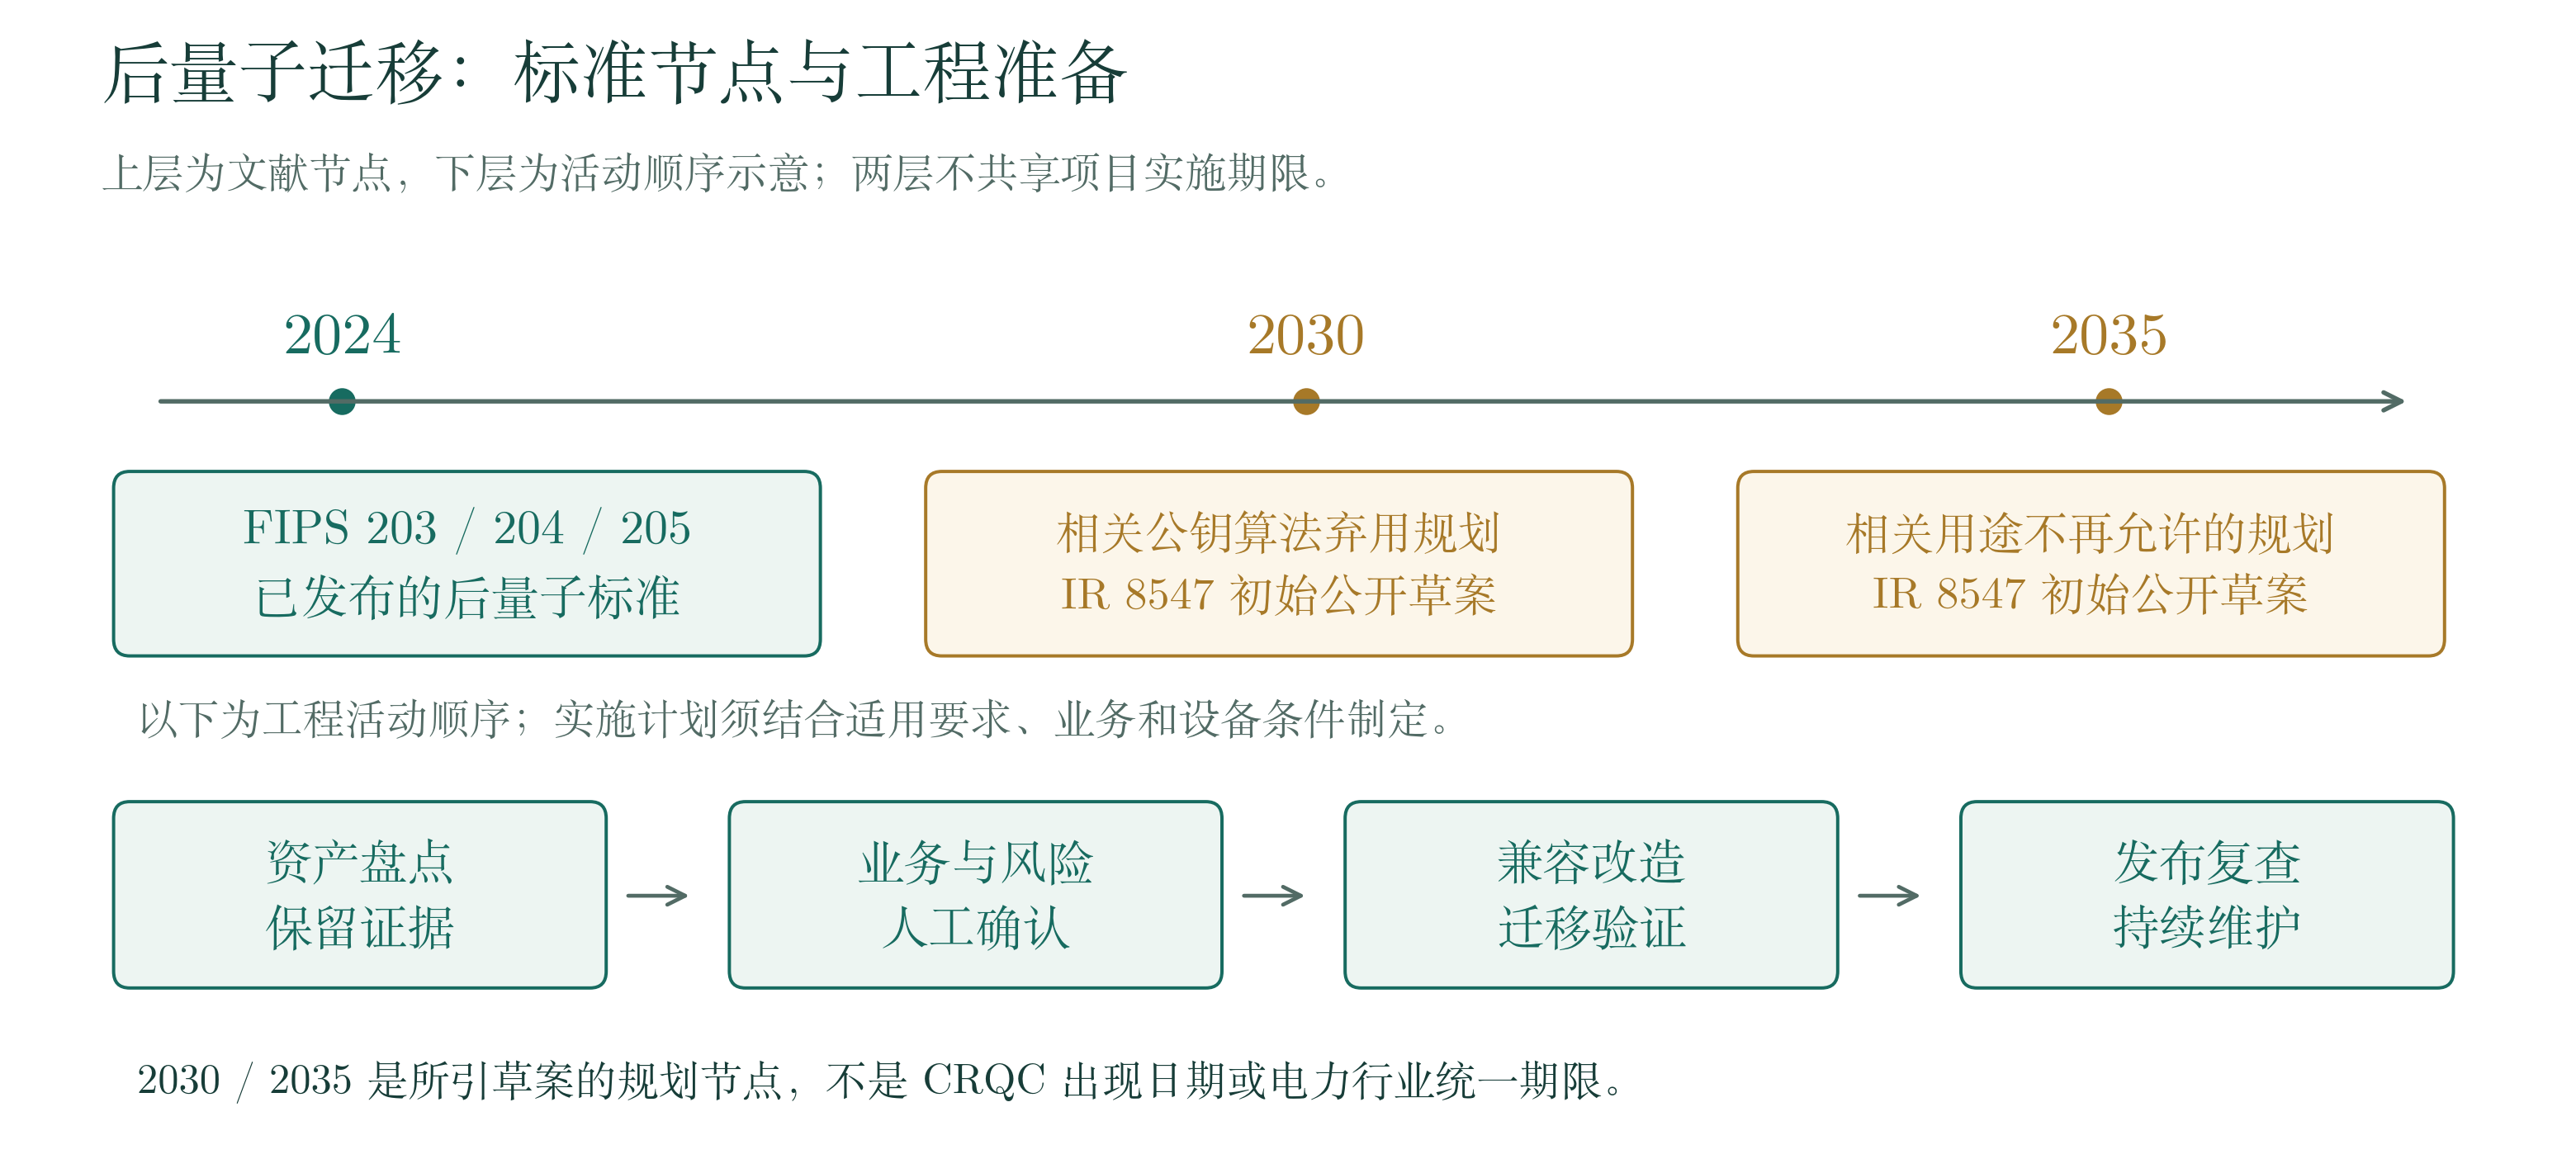
\includegraphics[width=\linewidth]{19-post-quantum-migration-timeline.png}
    \caption{后量子标准与迁移准备活动的时间关系示意。2030 与 2035 节点来自 NIST IR 8547 初始公开草案\cite{nistir8547}，不是量子计算机到来日期或电力行业统一期限。}
    \label{fig:pqc-timeline}
\end{figure}

\subsection{电力领域密码的重要性与识别的紧迫性}

电力系统是关乎国计民生的关键信息基础设施，密码技术在发电、输电、变电、配电、用电各环节深度应用，其作用不止于防止数据被窃取，还关系到控制指令真实性、软件升级可信性与电网运行稳定性。密码机制失效可能带来遥控遥调指令伪造、保护定值篡改、量测数据失真与用户信息泄露等风险。我国《电力监控系统安全防护规定》已于 2024 年修订，并自 2025 年 1 月 1 日起施行\cite{dianli27}。防护体系中的身份认证、安全传输与访问控制等环节高度依赖密码能力，因此开展资产盘点具有明确业务背景。表~\ref{tab:power-crypto-deployment} 给出各环节的典型应用形态；其中算法为业务分析示例，不代表所有实际设备采用相同配置，也不表示本文已经扫描这些现场系统。承担\textbf{身份认证与密钥分发}职能的传统公钥机制分布于多个业务链路，少量抽样难以代替系统性的资产清单与持续维护。

\begin{table}[htbp]
    \centering
    \caption{电力系统各环节的密码应用形态}
    \label{tab:power-crypto-deployment}
    \small
    \begin{tabularx}{\linewidth}{@{}p{1.9cm}p{3.4cm}p{3.0cm}X@{}}
        \toprule
        \textbf{业务环节} & \textbf{典型密码应用形态} & \textbf{涉及算法} & \textbf{迁移关注} \\
        \midrule
        调度与控制 & 纵向加密认证装置、调度数字证书系统 & SM2、RSA、SM3、SM4 & 需评估公钥迁移 \\
        \midrule
        变电站自动化 & 站控层通信安全、装置身份认证 & SM2、RSA、SM3、SM4、AES & 需评估公钥迁移 \\
        \midrule
        配电自动化 & 配电终端接入认证、遥控指令保护 & SM2、SM4 & 需评估公钥迁移 \\
        \midrule
        用电信息采集 & 采集终端安全模块、主站密钥管理 & SM4、SM2、AES & 需评估公钥迁移 \\
        \midrule
        新能源与储能 & 场站控制器通信、功率控制指令认证 & SM2、TLS 相关算法 & 需评估公钥迁移 \\
        \midrule
        运维与管理 & 运维通道 TLS/SSH、主机存储加密 & RSA、ECDSA、AES、SHA-2 & 需评估公钥迁移 \\
        \bottomrule
    \end{tabularx}
\end{table}

电力密码资产在分布上高度碎片化：终端类型至少涵盖变电站智能电子设备（IED）与测控装置、配电自动化终端（DTU/FTU/TTU）、智能电表与用电信息采集终端、纵向加密认证装置与安全接入网关、调度主站与服务器、新能源场站控制器及充电桩等；算法上既有 RSA、ECDSA、AES、SHA-2 等国际算法，也有 SM2、SM3、SM4 等国密算法，且常以混合方式并存。造成"底数不清"的技术根源有四：一是\textbf{密码与业务深度融合}，IEC 61850、DL/T 634.5104、用电信息采集等协议构成业务通信背景，其信道与管理通道可能另外部署密码安全机制\cite{iec61850,dlt634}，观察到业务流量并不等于识别出密码算法；二是\textbf{算法对上层不可见}，终端通过安全模块或安全装置提供密码能力，配置中往往只记录"启用加密"，而不记录所用算法与密钥长度；三是\textbf{多厂商、长周期的存量设备}在载体形态与实现方式上差异极大，缺乏统一的资产台账；四是\textbf{存量终端不一定具备主动上报密码配置的能力}，人工核查效率低、覆盖不全且更新滞后。上述根源共同导致电力系统的密码资产底数不清、量子脆弱性无法被全面发现，说明仅靠人工梳理难以持续支撑抗量子密码迁移这一系统性工程。

电力领域量子脆弱性识别的紧迫性来自三重因素的叠加：其一是\textbf{部分数据需要长期保密}，用户隐私、运行资料等应按业务要求评估保密期限，并据式~\eqref{eq:mosca} 分析迁移窗口；其二是\textbf{迁移周期长}，设备升级受检修窗口、备品备件、兼容性与厂商支持周期制约，需要尽早明确迁移对象与优先级；其三是\textbf{识别方式存在覆盖边界}，网络、配置和证书清点能够看到外部暴露属性，却不一定覆盖未启用功能、静态链接密码库和离线固件内部实现。由此需要形成系统性密码清单，在不干扰生产业务的条件下，结合离线证据与人工用途确认支撑迁移准备，而不能仅凭算法名称给出完整业务风险结论。

综合上述分析，本课题的目标是研制一款面向电力软件的密码资产识别与量子迁移辅助工具，实现可取得软件工件中的密码资产自动发现、算法识别与证据展示，并用组件溯源、风险提示及检测报告辅助人工分析。依据竞赛命题，作品面向四项量化目标展开：识别不少于 5 种密码算法，覆盖不少于 5 类电力终端，支持固件镜像、可执行程序等不少于 3 类检测对象，算法识别准确率不低于 90\%。本文采用有业务差异的五类终端软件场景开展验证，准确率、召回率与漏报率按明确的样本及标签口径分别报告。完整电力协议解析、自动业务风险评分、真实厂商终端与现场验证属于后续扩展方向。后续章节围绕上述目标介绍预备知识、方案设计与实验结果。

\section{国内外研究概况}

量子脆弱性识别在方法上涉及“密码资产发现”与“迁移风险分析”两个相互衔接的方向。国内外相关工作可沿三条线索梳理：密码资产发现的方法与数据表达，面向封闭软件的密码算法识别技术，以及能源行业与我国的应用要求。

\subsection{密码资产发现与迁移管理}

国际迁移实践普遍强调先发现密码使用位置，再评估影响并规划替换。NIST 国家网络安全卓越中心（NCCoE）的后量子迁移项目将\textbf{密码发现}（cryptographic discovery）作为重要工作内容，讨论通过多种发现方式构建组织范围密码清单的实践\cite{nccoe180038}。网络发现、端点与文件分析、应用与配置清点各自提供部分视图，需要保留来源和盲区。在数据表达方面，CycloneDX 1.6 引入密码学物料清单（Cryptography Bill of Materials，CBOM），为算法、协议、证书及相关密码属性提供结构化描述\cite{cbom16}。由此可形成“发现证据—结构化清单—用途确认—迁移建议”的管理链路。

工具生态既包括 IBM Quantum Safe 等企业密码发现与迁移管理方案，也包括 CBOMkit 等开源实践\cite{ibm-quantum-safe,cbomkit}。面向网络服务的发现适合了解协议和证书的外部暴露属性，源码与文件分析则有助于定位具体组件。二者不能互相替代：库内存在某种算法不表示业务已经使用，未从网络观察到某种算法也不表示发布包中不存在。本作品沿用资产发现与迁移辅助的思路，把主要工作范围放在可以取得的源码、程序与固件组件。

\subsection{封闭软件中的密码算法识别}

对于固件镜像、可执行程序等封闭对象，识别需要跨越符号缺失、编译优化与架构差异。Gr{\"o}bert、Willems 与 Holz 的研究讨论了二进制程序中密码原语的自动识别\cite{groebert2011}；2024 年 ACSAC 的系统研究进一步比较了二进制密码函数识别方法\cite{acsac24}。这些工作表明密码实现具有可分析的程序特征，也说明实验结论必须结合参考实现、构建条件与评价对象理解，不能将已知库上的识别率直接解释为未知软件的通用覆盖能力。


\paragraph{名称、字节特征与已知实现识别}
源码名称和文本关键词方法成本较低，Wind River crypto-detector 提供了相关开源实践\cite{wind-detector}。
其限制是注释、声明、普通字符串与实际调用可能包含同样的文本，因此本工具补充词法掩盖和角色判定。
YARA 适合表达常量、查表和指令片段规则\cite{yara-docs,crypto-rules}；
规则在优化、硬件加速或不同字节序下可能失效，共享常量也可能产生混淆。
已知函数签名通过覆盖完整函数、处理重定位并核对常量增强依据，
但其适用域受参考库、编译器、优化等级与架构限制。

\paragraph{结构化分析、运算语义与固件接入}
ELF/PE 结构化解析可区分导入和定义，避免把链接密码库解释为拥有库内全部算法。
Tree-sitter 提供源码语法树，Capstone 提供跨架构反汇编\cite{tree-sitter,capstone}。
本作品在上述表示上构建位运算、查表、轮函数和部分大数关系的见证，
用数据依赖约束补充名称或字节完全匹配的不足。
Unicorn 用于隔离的有限指令探针\cite{unicorn}，不是运行完整业务程序。
Miasm 提供机器语义与中间表示\cite{miasm}，但中间表达式数量并不等于完整密码算法证据。
固件提取是另一类问题：Binwalk 提供格式识别和历史提取路线\cite{binwalk-v2}，
当前工程另有原生 SquashFS、gzip 与受限 ESP 适配器，提取后复用统一扫描入口。

\begin{table}[htbp]\centering\small
\caption{主要方法的作用与限制；本表为技术比较，非同条件性能排名}\label{tab:method-comparison}
\begin{tabularx}{\linewidth}{p{2.4cm}p{4.4cm}X}\toprule
方法 & 适合解决的问题 & 主要限制\\\midrule
名称/接口 & 定位明确 API 和动态导入 & 名称可删除或变化；引用不证明实现或执行。\\
字节/常量 & 低成本定位标准表和轮常量 & 共享表、优化与字节序影响；需排除纯数据诱饵。\\
已知函数 & 核验已审核实现的完整字节与角色 & 已见库与构建覆盖有限，不能外推未知家族。\\
运算图/语义 & 识别不依赖变量名的数据依赖 & 路径、内存、调用与预算限制明显。\\
固件组件 & 把镜像关联到可定位的组件证据 & 加密区域、未知文件系统与外部硬件仍未知。\\\bottomrule
\end{tabularx}\end{table}


\subsection{能源行业与国内应用要求}

能源行业的密码迁移必须结合控制业务、安全分区、装置寿命与供应链协同。IEC 62351 系列覆盖电力数据和通信安全，IEC 61850 等标准提供业务通信背景\cite{iec62351,iec61850}。对相关系统的量子风险分析，需要把算法、证书、协议配置与实际业务用途关联起来。网络通道的安全试点或单一协议替换，都不能自动说明存量软件中全部密码能力已经完成清点。离线发布包分析可补充其中的软件证据，但不能代替装置测试与生产环境评估。

国内密码应用还受到国密算法标准与商用密码应用要求的约束。SM2、SM3、SM4 已有相应国家标准\cite{gbt32918,gbt32905,gbt32907}，GB/T 39786 与 GM/T 0054 等给出信息系统密码应用的基本要求\cite{gbt39786,gmt0054}。这类要求为身份鉴别、机密性、完整性和密钥管理等提供评估依据；后量子迁移还需要进一步考察算法的量子计算风险、替换兼容性与生命周期。满足既有合规要求与完成后量子迁移是需要分别验证的目标。

综合来看，本文重点处理三项工程问题：一是补充源码、二进制与固件之间的离线证据关联；二是区分接口引用、实现包含及尚未确认的运行时使用，避免把算法列表直接当作业务风险结论；三是在资源受限条件下，将识别证据组织为可复核资产清单，支持用途核查和迁移准备。对电力专有协议的完整解析，以及结合数据保密期、资产关键性的自动风险排序，仍需后续研究。

\clearpage
\section{作品功能与性能说明}
本作品面向电力软件交付与运维核查，由密码识别引擎、固件提取模块和本地工作台组成。用户提交文件或目录后，工具识别对象类型并执行检测，生成密码资产清单和原始证据，供用户核对密码用途、规划迁移。检测以离线静态分析为主。

源码分析支持 C/C++ 与部分 JavaScript 代码，定位密码接口调用及实现证据。程序分析面向 Linux 与 Windows 程序及共享库，记录符号和文件偏移。固件先提取内部文件，再逐组件分析并记录来源，失败或预算超限的部分单独标记。

当前支持十三种算法，包括对称加密算法 AES 和 SM4、摘要算法 SHA-256 和 SM3，以及 RSA 和 SM2 等公钥算法。智能电能表、采集集中器、馈线终端、保护装置和边缘网关五类软件样例已用于验证。十份面向两种处理器架构的自制镜像共恢复 650 个文件，其中 540 个为二进制文件，530 个文件包含密码实现，验证范围限于软件流程。

工作台可通过文件或文件夹上传、服务器路径和内置样例创建任务，查看处理阶段与历史记录，支持结果搜索和筛选。用户可核对源码行号、程序偏移及组件内容摘要，查看算法类别对应的量子风险提示与迁移建议。页面区分密码接口引用与文件内实现，局部线索留待复核，静态结果不证明实际启用。报告可导出为结构化数据、表格文件和文本，保留原始证据。命令行入口也可直接提交本地文件或目录。

既有评测使用 1071 份源码与两种架构的程序，一份文件与一种算法组成一项判定，重复证据合并计数。747 项实现标注中正确检出 726 项，漏检 21 项，没有范围内误报。计入 11206 项正确排除结果后，准确率为 99.82\%，实际存在算法的检出比例，即召回率为 97.19\%。样本参与过规则与参考库修订，结果仅说明已知实现覆盖。

耗时测量采用 Xeon Silver 4410Y 处理器、Fedora CoreOS 42 系统与 Python 3.12.3 环境，源码与程序串行测量，各类扫描均关闭可选语义后端。源码与程序沿用八份固定样本，各预运行一次再测三次；固件记录十份镜像在三个任务并发下各扫描一次的耗时，分别汇总范围。计时含进程启动、分析和报告写出，固件另含解包，不含网页交互，仅反映所测小样本表现。

\begin{table}[htbp]\centering\small
\caption{三类检测对象的文件大小与实测耗时范围}\label{tab:implemented-scope}
\begin{tabularx}{\linewidth}{@{}Xrr@{}}\toprule
检测对象 & 文件大小范围（字节） & 耗时范围（秒）\\\midrule
源码文件 & 329--1464 & 0.193--0.356\\
程序文件（共享库） & 33416--72032 & 3.012--3.884\\
固件镜像 & 3981312--4132864 & 93.208--133.740\\\bottomrule
\end{tabularx}
\end{table}

\clearpage
\section{创新性说明与优势分析}
本作品针对电力软件中密码功能分散于不同文件与组件的特点，将源码、可执行程序和固件镜像纳入统一检测流程。设计重点在于明确算法识别的判定条件，并建立识别依据与文件位置之间的对应关系，支持识别结果的定位与复核。

源码中的算法名称可能出现在注释、函数声明或调用表达式中，仅凭名称匹配难以区分其含义。本文结合词法处理与局部语法判定，区分接口名称的声明、定义与调用，将接口引用判定建立在调用及参数依据之上，并保留其在原始源码中的位置。对于通用密码接口，依据调用处明确给出的选择参数确定具体算法，参数取值无法确定时则保留待确认状态，从而减少注释及同名声明等无关文本的干扰。

对于缺少函数名称等符号信息的可执行程序，本文在 YARA 初步特征匹配\cite{yara-docs}的基础上，进一步对照固定版本开源密码库中的完整函数进行核验。核验时仅对预先审核的地址变化作匹配调整，并检查函数引用的常量及所需的关键运算。仅发现局部相似片段时，结果保留为待确认线索，满足完整核验条件后才作为算法实现的依据。匹配记录同时保留参考库版本、编译条件及核验依据，便于对照具体参考代码复查结果；匹配范围仍受已收录构建条件限制。

在程序指令分析中，本文利用 Capstone 反汇编引擎\cite{capstone}解析程序指令，并以可选的 Miasm 二进制分析框架\cite{miasm}辅助表示和分析指令中的运算关系。分析过程记录参与运算的数据来源、处理位数及前后计算关系。即使操作种类和常量相同，数据来源或计算关系不同，也可能对应不同的计算过程。保留这些信息能够区分部分表面相似的代码，为名称识别和固定代码匹配提供补充。

证据复核方面，本文将外层镜像、内部组件与算法位置建立对应关系，保留内容摘要及提取来源。软件发布包发生变化时，分析人员可据此确认发现属于哪个组件，并回到原始文件核对。复核对象由此明确到具体交付文件，便于按组件检查密码资产，其覆盖仍依赖实际提取结果。

针对多个业务系统共用密码组件时迁移影响范围难以确定的问题，本文借鉴图检索增强生成（GraphRAG）\cite{graphrag2024}的实体关系组织方法，提出结合关联图与本地大模型的扩展方案。该方案拟记录终端、业务系统与密码组件之间的使用关系，在分析组件替换或升级时，通过图检索向模型提供相关记录及依赖路径，辅助梳理可能受到影响的终端与业务。模型拟在本地部署，以减少软件代码和业务资料向外部服务传输的需求，降低敏感信息外传风险。该方案尚未完整实现，关联分析效果及运行开销仍需后续验证。
